
\newpage

\section*{Annexe 2}
\textbf{Notations}

La base $\bas{0}$ associée au repère $\rep{0}$ est notée $\repere{O}{x_0}{y_0}{z_0}$. Il en est de même pour le repère $\rep{1}$ associé au bras 1 et pour le repère $\rep{H1}$ associé à l’hélice $H1$. On note :
\begin{itemize}
\item $\ell$ et $L$, respectivement la largeur et la longueur du parallélépipède rectangle englobant
la totalité du drone (représenté en pointillés sur la \autoref{fig:23}), de hauteur $h = \SI{115}{mm}$,
constante quelle que soit la configuration du drone;
\item $L_0 = \SI{280}{mm}$, la longueur du corps 0;
\item $\vect{­OA_1} = \dfrac{L_0}{2} \vx{0} + \dfrac{h}{4}\vz{0}$;
\item $L_1 = \SI{140}{mm}$, la longueur du bras 1;
\item $\vect{I_1A_1} = \dfrac{L_1}{2} \vx{1} - \dfrac{h}{4} \vz{0}$;
\item $r_h = \SI{64}{mm}$, la longueur d’une pale de l’hélice;
\item $\vect{I_1 P} = r_h \vect{x_{H1}}$ pour l’hélice H1.
\end{itemize}

\begin{figure}[H]
\centering
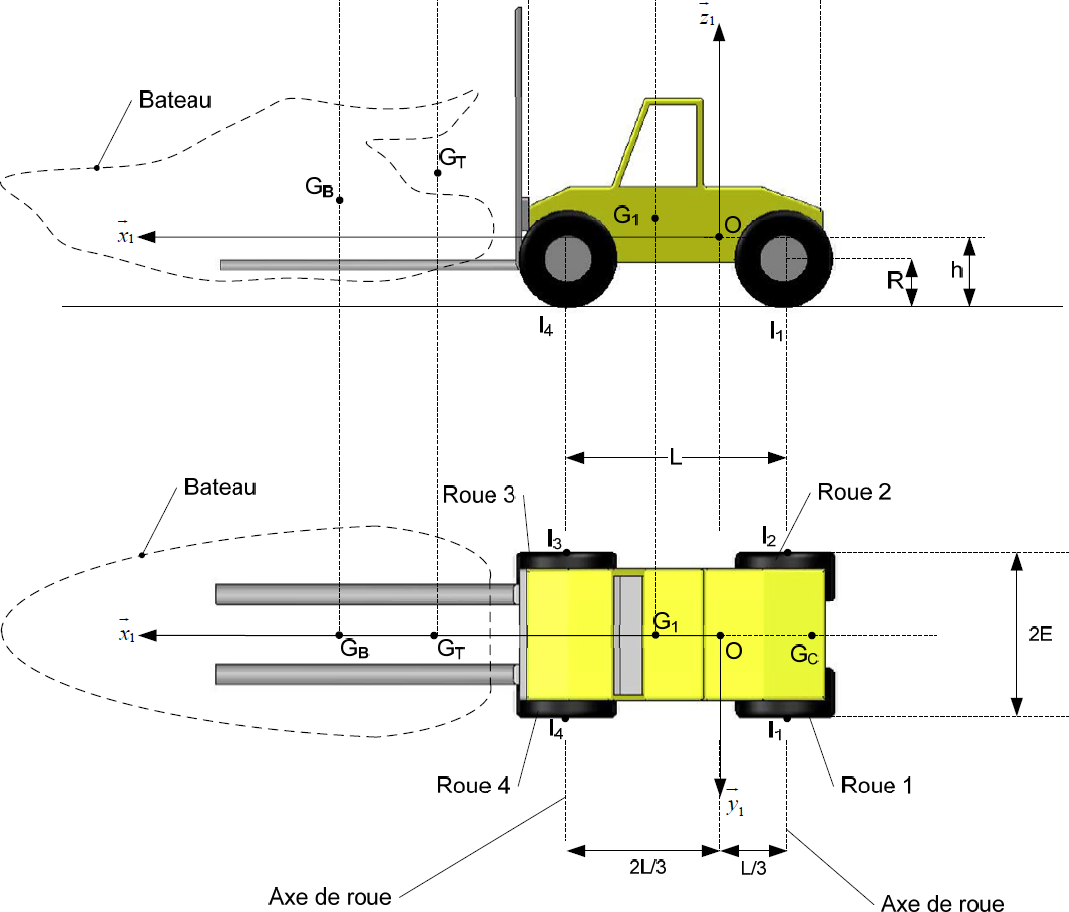
\includegraphics[width=\linewidth]{fig_23}
\caption{\label{fig:23}  Vue de dessus et en perspective du drone en phase de repliement et paramétrage de la géométrie}
\end{figure}


\begin{figure}[H]
\centering
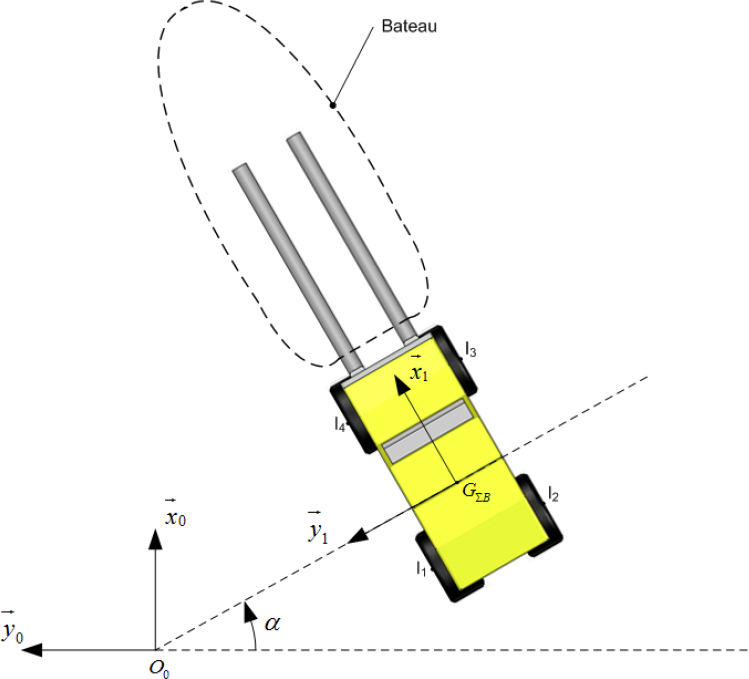
\includegraphics[width=.5\linewidth]{fig_24}
\caption{\label{fig:24} ­ Figures planes du paramétrage du bras $i$ par rapport au corps 0 du drone et de
l’hélice $H1$ par rapport au bras 1 du drone}
\end{figure}



\section*{Annexe 3}

Les matrices d’inerties des principaux éléments du drone, dont la géométrie a été simplifiée
pour cette étude, sont données ci­dessous, chacune dans la base principale d’inertie :

Pour le corps 0, de centre d’inertie O et de masse $m_c$ : $\inertie{0}{O} = \matinertie{I_{cx}}{I_{cy}}{I_{cz}}{0}{0}{0}{O,\bas{0}}$.

Pour le bras 1, de centre d’inertie $A_1$ et de masse $m_b$ : $\inertie{1}{A_1} = \matinertie{I_{bx}}{I_{by}}{I_{bz}}{0}{0}{0}{A_1,\bas{1}}$.

Pour le bras 2, de centre d’inertie $A_2$ et de masse $m_b$ : $\inertie{2}{A_2} = \matinertie{I_{bx}}{I_{by}}{I_{bz}}{0}{0}{0}{A_2,\bas{2}}$.

Pour chaque hélice $H_i (i = 1 à 4)$, de centre d’inertie $I_i$ et de masse $m_h$, le moment d’inertie
selon l’axe $\axe{I_i}{z_0}$ est noté $I_{hz}$.

On note $\Sigma$ l’ensemble constitué des principaux éléments du drone, tel que $\Sigma = \left\{ 0+1+2+\sum_{i=1}^{4}H_i \right\}$.



\section*{Annexe 4}


\begin{figure}[H]
\centering
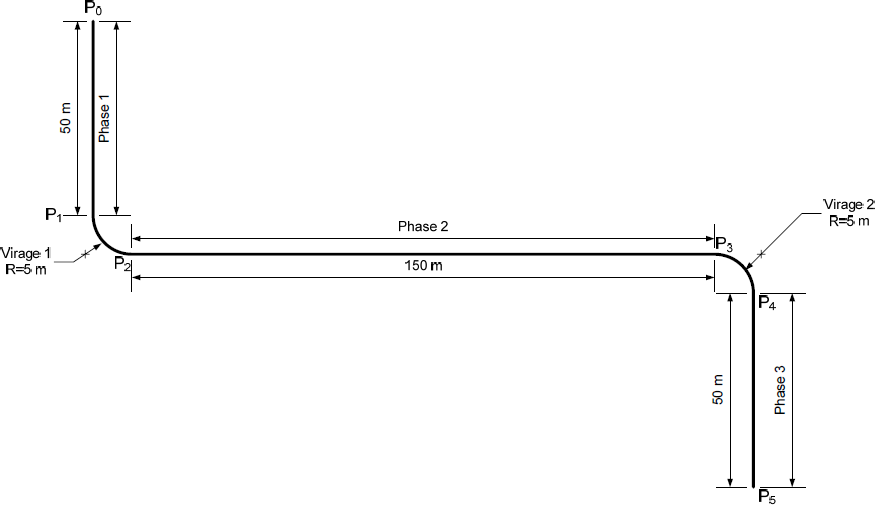
\includegraphics[width=.4\linewidth]{fig_25}
\caption{\label{fig:25} Mécanisme de mise en mouvement du bras}
\end{figure}

\textbf{Notations}
\begin{itemize}
\item l’orientation de la poulie 5 par rapport au corps du drone 0 est paramétrée par l’angle
$\theta(t)$ tel que : $\theta(t)(t) = \left(\vx{0},\vx{5}\right) = \left(\vy{0},\vy{5}\right)$;
\item­ le rayon d’enroulement du câble métallique 1 sur la poulie 5 est noté $R_1$, avec
$R_1 = \SI{30}{mm}$. Ce rayon d’enroulement correspond à la distance $OC_1$, tel que $\vect{OC_1}= R_1\vy{0}$;
\item­ en première approximation et afin de simplifier la géométrie pour l’étude de la loi entrée
/ sortie de ce mécanisme, on considère la longueur $B_1C_1$ telle que $\vect{C_1B_1} = L_{c1}(\theta) \vect{x_{c1}}$, avec $L_{c1}(\theta) = L^{\text{init}}_{c1} - R_1\theta$. La grandeur $L^{\text{init}}_{c1}$ correspond à la distance $B_1C_1$ pour $\gamma_1 = 90\degres$, on a
alors le point $P_1$ confondu avec $C_1$ et $\theta = 0\degres$;
\item­ la distance du point d’accroche $B_1$ du câble métallique 1 sur le bras 1 est notée $a_1$ telle
que $\vect{A_1B_1} = -a_1 \vx{1}$, avec $a_1 = \SI{40}{mm}$;
\item­ la distance du point d’accroche $B_2$ du câble métallique 2 sur le bras 2 est notée $a_2$ telle
que $\vect{A_2B_2} = a_2 \vect{x_2}$, avec $a_2 = a_1 = \SI{40}{mm}$;
\item­ on rappelle que $\vect{OA_1} = \dfrac{L_0}{2}\vx{0}$  avec $L_0 = \SI{280}{mm}$.
\end{itemize}

On considère la position initiale du mécanisme, en configuration bras dépliés, telle que
$\gamma_1= 90\degres$ et $\gamma_2 = 90\degres$ et donc $\theta = 0\degres$. On a alors $L_{c1}(\theta = 0\degres) = L^{\text{init}}_{c1}$ et $L_{c2}(\theta = 0\degres) = L^{\text{init}}_{c2}$.

La position finale du mécanisme est la position pour laquelle les bras sont alignés avec la
direction prépondérante du drone, c’est­à-dire pour $\vx{1} = \vx{0}$ et $\vx{2} = -\vx{0}$. On a alors $\gamma_1 = 0\degres$, $\gamma_2 = 180\degres$ et $\theta = \Delta \theta$, où $\Delta \theta$ est la course angulaire de la poulie avec $L_{c1}(\Delta \theta) = L^{\text{final}}_{c1}$ et
$L_{c2}(\Delta \theta) = L^{\text{final}}_{c2}$.